\documentclass{school-22.101-notes}
\date{October 17, 2011}

\begin{document}
\maketitle


%%%%%%%%%%%%%%%%%% New Part: Nuclear Structure %%%%%%%%%%%%%%%%%%%%%%%%%%%%%%%%%
\lecture{Bound State of A Deuteron, Finite Square Well\label{2H-bound-state}}
Reference: Liboff 10.5, Krane 4.1, 4.2, 4.4.

We have solved the simple finite square well problem in Chapter~\ref{finite-square-well} (recall the even parity and odd parity cases). Now we consider the simplest bound state nucleus: a deuteron \ce{^2H}. Basics about the deuteron: 
\begin{itemize}
\item \ce{^2_1 H_1} is consist of a neutron and a proton. 
\item Its nuclear radius is 2.1 fm. 
\item The binding energy of a deuteron is, 
  \eqn{ (m(n) + m(\ce{^1H}) - m(\ce{^2 H})) c^2 = 2.22 \MeV} 
  which is very small compare with other particles. This is the lowest point on a B/A vs. A curve (generating a 1.11 MeV/A point, where the maximum is about 8 MeV/A). 
\end{itemize}

We will show that a bound state problem can be reduced into three components:
\begin{enumerate}
\item An eigenvalue problem (Section \ref{2H-eigenvalue});
\item An analytical relation and a quantitative relation between $V_0, \Gamma_0, E_0$ (Section \ref{2H-relation});
\item The spin dependence of the nuclear force (Section \ref{2H-spin}).
\end{enumerate}



\topic{Reduce Bound State Problem into Eigenvalue Problem \label{2H-eigenvalue}} 
\begin{enumerate}
\item Write out the Hamiltonian: 
\eqn{ \Hhat = \frac{1}{2 m_n} \phat_n^2 + \frac{1}{2 m_p} \phat_p^2 + V_{\mathrm{nuc}} (\uline{x}_n - \uline{x}_p ) }
in which 
\begin{align}
 V_{\mathrm{nuc}} (\uline{x}_n - \uline{x}_p ) &= \mbox{Potential interaction (only depends on the radial distance b/w the two particles)} \\
 (\uline{x}_p, \phat_p; \uline{x}_n, \phat_n) &= \mbox{State vectors of the two particles} 
\end{align}
We assume central potential. 6-degrees of freedom = \# of coordinates in the state vector

\item Define Center-of-Mass (COM) frame: 
\eqn{
 H &\to H_{\mathrm{CM}} + H_{\mathrm{Rel}}, 
&(\uline{x}_p, \uline{p}_p; \uline{x}_n, \uline{p}_n) &\to (\uline{r}, \uline{p}_{\mathrm{Rel}}; \uline{R}, \uline{p}_{\mathrm{CM}} ) 
}
\begin{align}
\begin{dcases*} 
\uline{R} = \frac{1}{m_n + m_p} (m_p \uline{x}_p + m_n \uline{x}_n ) & C.M. position\\
\uline{r} = \uline{x}_p - \uline{x}_n & Relative position \\
\uline{p}_{\mathrm{CM}} = \uline{p}_{n} + \uline{p}_p & Momentum of CM \\
\uline{p}_{\mathrm{Rel}} = \frac{m_p \uline{p}_n - m_n \uline{p}_p}{m_n + m_p} & Momentum of coordinate relative to C.M \\
\end{dcases*}
\end{align}

\item With some math, we can transform the $(n,p)$ two body problem into an effectively single particle eigenvlaue problem: 
\begin{align}
[\derivative \vec{R}, \derivative \vec{r}] &= [ \derivative \vec{x}_n \derivative \vec{x}_p] \left[ \begin{array}{cc} 
\frac{m_n}{m_n + m_p} & -1 \\ 
\frac{m_p}{m_n + m_p} & 1 
\end{array} \right]   \\
f(\vec{R}, \vec{r}) &= [ \derivative \vec{x}_n, \derivative \vec{x}_p]  \left[ \begin{array}{c} \uline{\gradient}_n \\ \uline{\gradient}_p \end{array} \right] f(x_n, x_p)  \\
&= [ \derivative \vec{R}, \derivative \vec{r}]  \left[ \begin{array}{c} \uline{\gradient}_R \\ \uline{\gradient}_r \end{array} \right] f(x_n, x_p)  
\end{align}
\begin{align}
\Rightarrow 
\left[ \begin{array}{cc} 
\frac{m_n}{m_n + m_p} & -1 \\ 
\frac{m_p}{m_n + m_p} & 1 
\end{array} \right]   
\left[ \begin{array}{c} \uline{\gradient}_R \\ \uline{\gradient}_r \end{array} \right] 
&=  \left[ \begin{array}{c} \uline{\gradient}_n \\ \uline{\gradient}_p \end{array} \right]
\end{align}
We plug into our original definition of $K$: 
\begin{align}
K &= - \frac{\hbar^2 \uline{\gradient}_n^2}{2 m_n}  - \frac{\hbar^2 \uline{\gradient}_p^2}{2 m_p}  \\
&= - \frac{\hbar^2}{2} [ \uline{\gradient}_n, \uline{\gradient}_p] \left[ \begin{array}{cc} \frac{1}{m_n} & 0 \\ 0 & \frac{1}{m_p} \end{array} \right] \left[ \begin{array}{c} \uline{\gradient}_n \\ \uline{\gradient}_p \end{array} \right] \\
 &= - \frac{\hbar^2}{2} [ \uline{\gradient}_R, \uline{\gradient}_r] 
\left[ \begin{array}{cc} \frac{m_n}{m_n+m_p} & \frac{m_p}{m_n+ m_p} \\ -1 & 1 \end{array} \right]
\left[ \begin{array}{cc} \frac{1}{m_n} & 0 \\ 0 & \frac{1}{m_p} \end{array} \right] 
\left[ \begin{array}{cc} \frac{m_n}{m_n+m_p} & -1 \\ \frac{m_p}{m_n+ m_p} & 1 \end{array} \right]
\left[ \begin{array}{c} \uline{\gradient}_R \\ \uline{\gradient}_r \end{array} \right] \\
&= - \frac{\hbar^2 \laplacian_R}{2 (m_1 + m_2)} - \frac{\hbar^2 \laplacian_r}{2 \mu} \\
&= - \frac{\hbar^2 \laplacian_R}{2M} - \frac{\hbar^2 \laplacian_r}{2 \mu} = \frac{P^2}{2M} + \frac{p^2}{2\mu} 
\end{align}
where $\mu$ is the reduced mass, $M$ is the total mass. So we have reduced a two body problem into  a single particle (the reduced mass) about the center of mass (where $B$ is the binding energy in the two-body problem): 
\eqn{ \Hhat \psi(\vec{r}) &= - \vec{B} \psi(\vec{r}) }
% \eqn{\Rightarrow e^{i \uline{K} \cdot \uline{R}} \psi(\uline{x}) &= \psi(\uline{x}_1 - \uline{x}_2) }

\item We ignore the COM translation, and focus on a stationaty deuteron. 
\begin{align}
\Hhat_d &= \overbrace{\frac{\uline{\Phat}_{\mathrm{CM}}^2}{2M}}^{ = \hat{E}_{\mathrm{CM}} \to  0} + \frac{\uline{\Phat}_{\mathrm{Rel}}^2}{2\mu} + V_{\mathrm{nuc}} (\uline{r}) = \frac{\uline{\Phat}_{\mathrm{Rel}}^2}{2\mu} + V_{\mathrm{nuc}} (\uline{r}) = -\frac{\hbar^2}{2 \mu} \gradient_r^2 + V_{\mathrm{nuc}} (\uline{r}) 
\end{align}

\item Now we perform a qualitative evaluation of $V_{\mathrm{nuc}} (\uline{r})$ \footnote{Krane, p.80}: 
    \begin{enumerate}
    \item At short distances: very strong, overcome the Coulomb repulsion of protons in the nucleus; 
    \item At long distances (on the order of atomic size): very week and negligible; 
    \item Some particles, like $e^-$, are immute to $V_{\mathrm{nuc}}$;
    \item The nucleus potential looks like Figure~\ref{nuclear-potential-radius}. 
    \begin{figure}
        \centering
        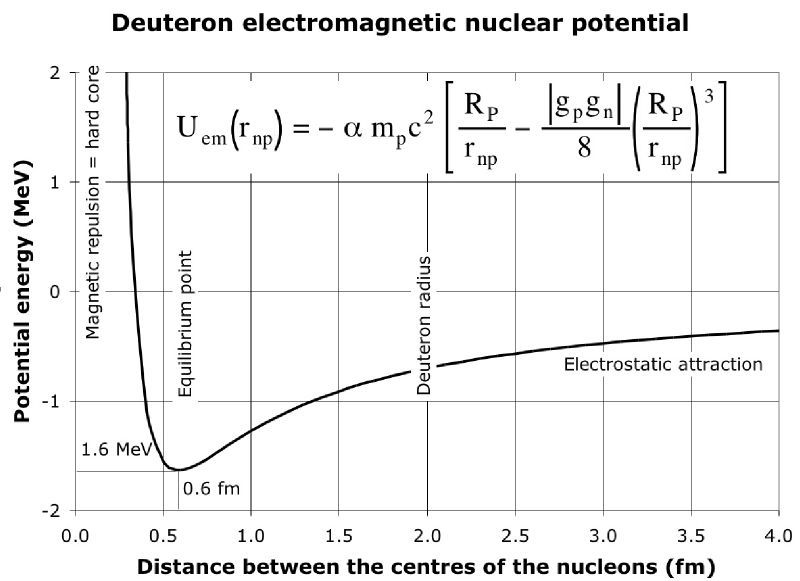
\includegraphics[width=3in]{images/deuteron/nuclear-potential-radius.png}
        \caption{Deuteron Electromagnetic Nuclear Potential\label{nuclear-potential-radius}}
    \end{figure}
    \end{enumerate}

\item A quantitative evaluation of $\uline{\gradient}_r^2$: 
\begin{align}
\uline{\gradient}_r^2 &= - \frac{L^2}{\hbar^2 r^2} + \frac{1}{r^2} \ddr \left( r^2 \ddr \right) \\
- \frac{\hbar^2}{2 \mu} \uline{\gradient}_r^2 &= - \frac{\hbar^2}{2 \mu} \left[ \pprn2 + \frac{2}{r} \ppr \right] + \frac{1}{2 r^2 \mu} \overbrace{ (-\hbar^2) \left[ \frac{1}{\sin \theta} \pptheta \left( \sin \theta \pptheta \right) + \frac{1}{\sin^2 \theta} \ppphin2 \right]}^{\to \Lhat^2}  \\
&= - \frac{\hbar^2}{2 \mu} \left[ \pprn2 + \frac{2}{r} \ppr \right] + \frac{\Lhat^2}{2 r^2 \mu} 
\end{align}
Basically we break the kinetics energy into a translatioal component and a rotational component. 

\item Now we have our eigenvalue problem ($E$'s sign is negative because of a bound state, and its magnitude is the binding energy of the deuteron in this case):
\eqn{ \left[ - \frac{\hbar^2}{2 \mu} \left( \pprn2 + \frac{2}{r} \ppr \right) + \frac{\Lhat^2}{2 r^2 \mu} + V_{\mathrm{nuc}} (\uline{r})  \right] \psi_n (r, \theta, \phi) = E_n \psi_n (r, \theta,\phi) }

\item To evaluate the above eigenvalue problem, notice we have
\eqn{ \left[ \Lhat^2, \Hhat \right]   = \left[ \Lhat_z , \Hhat \right] = 0 }
suggesting that $\Lhat^2, \Lhat_z, \Hhat$ shares the same eigenstate, which is the spherical harmonics $Y_l^m (\theta, \phi)$. Then we can write the wave function as:
\eqn{ \psi_n (r, \theta, \phi) = \psi_{n,l} (r) Y_l^m (\theta, \phi) }
Also we know 
\eqn{ \Lhat^2 Y_l^m = \hbar^2 l(l+1) Y_l^m }
Plug the eigenvalues of $\Lhat^2$ back into the eigenvalue problem: 
\eqn{ \left[ - \frac{\hbar^2}{2 \mu}\left( \pprn2 + \frac{2}{r} \ppr \right)  + \frac{\hbar^2 l(l+1)}{2 \mu r^2 } + V_{\mathrm{nuc}} (\uline{r}) - E_{n,l}  \right] \psi_{n,l} (r) Y_l^m (\theta, \phi) = 0 }
Notice that the above equation is only dependent on r, so we can cross out the $Y_l^m (\theta, \phi)$ term, and define $\displaystyle u_n(r) = r \psi_n (r)$,
 \eqn{  \boxed{ \left[ - \frac{\hbar^2}{2 \mu}  \pprn2  + \underbrace{\frac{\hbar^2 l(l+1)}{2 \mu r^2 } + V_{\mathrm{nuc}} (\uline{r}) }_{\to V_{\mathrm{eff}} (\uline{r})} - E_{n,l}  \right] u_n (r)  = 0 } }
This is the called the \textbf{radial equation}. It is identical in form to the 1D Schrodinger equatio, except that the effective potential $V_{\mathrm{eff}} (r)$ contains an angular momentum term, which is called the \textbf{centrifugal term}. The centrifugal term `tends to throw the particle outward (away from the origin), just like the centrifugal (pseudo-)force in classical mechanics' (Griffths, Section 4.1)\footnote{My understanding: we started out with both radial and angular dependency; after separation of variables, we solved for the angular dependency and reached the radial equation. Effectively we went from the earth reference frame into a rotating reference frame (that's the only way we don't see rotational movement anymore), thus we need to add a pseudo centrifugal force to account for the change in reference frame.}.    
\end{enumerate}

\clearpage
\begin{figure}
    \centering
    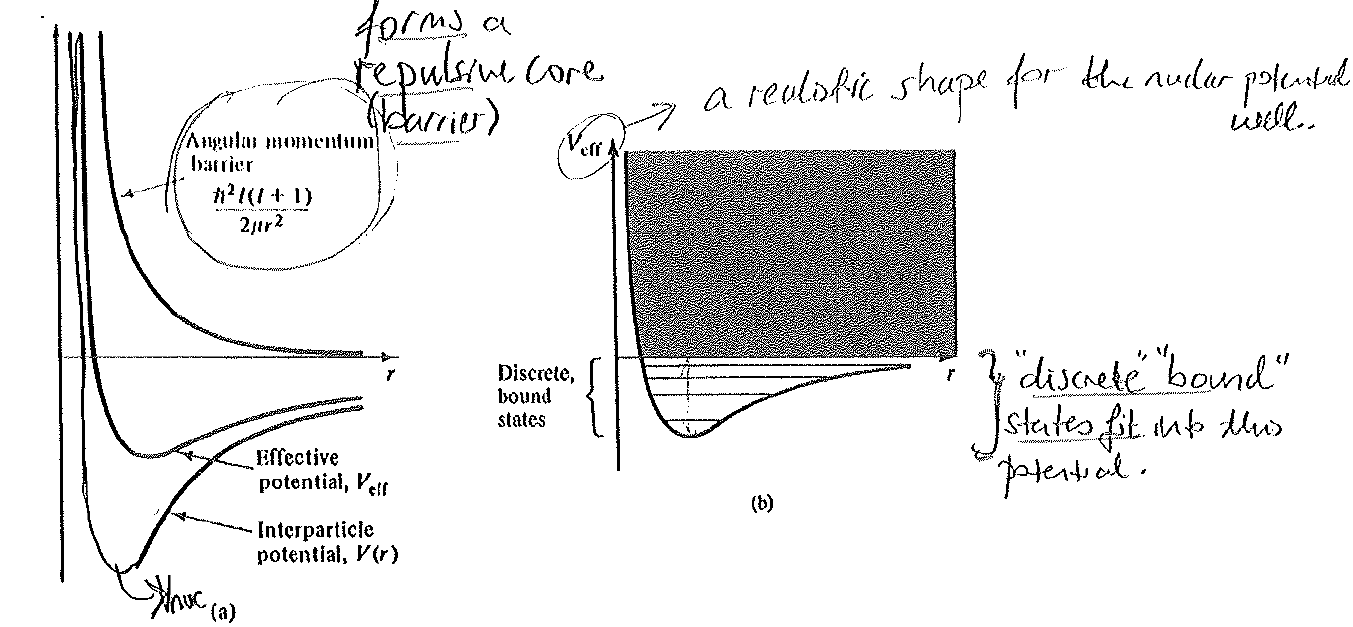
\includegraphics[width=5in]{images/deuteron/deutrium-V-eff.png}
    \\
    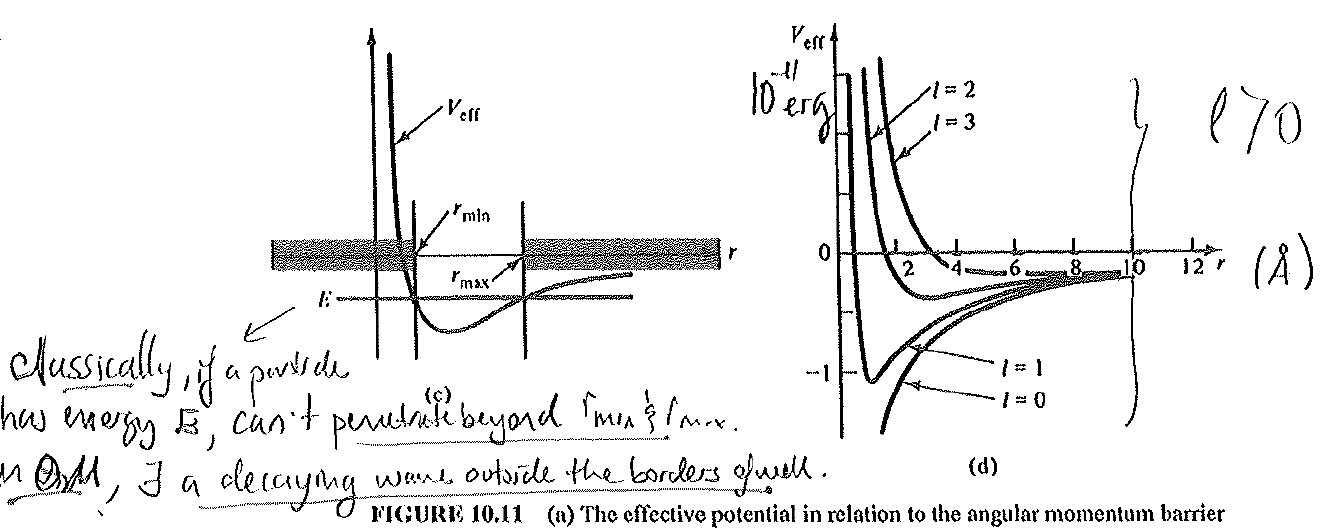
\includegraphics[width=5.5in]{images/deuteron/deutrium-V-eff-2.png}    
    \caption{$V_{\mathrm{eff}}$'s Effect on a Deutron}
    \label{V-eff}
\end{figure}
\textbf{How $V_{\mathrm{eff}}$ affects a deutron (Fig.~\ref{V-eff}):}
\begin{enumerate}
\item Original $V_{\mathrm{nuc}} (r)$ is mostly attractive (negative); 
\item Angular momentum terms act as a repulsive barrier as it is positive;
\item $V_{\mathrm{eff}} (r)$ is still mostly attractive (negative), but weaker than $V_{\mathrm{nuc}} (r)$. In a word, \textcolor{blue}{$V_{\mathrm{eff}}$ lifts the potential up from the original $V_{\mathrm{nuc}}$, making the interaction weaker;} 
\item There are discrete bound states that fit into the potential. 
\end{enumerate}

Next: We've defined the particle potential. Now we are looking for the permitted energy levels $E_n$ that can fill in the potential. If we have a weaker potential, we can fit in less energy levels. Vice versa. In the next sections we will solve this problem for deutrons. 
\end{document}
